\chapter{Transition Plugins}%
\label{cha:transition_plugin}

When one edit ends and another edit begins, the default behavior is to have the first edit's output immediately become the output of the second edit when played back. Transitions are a way for the first edit’s output to become the second edit’s output with different variations. The audio and video transitions are listed in the Resources window as figure~\ref{fig:transition}.

\begin{figure}[htpb]
    \centering
    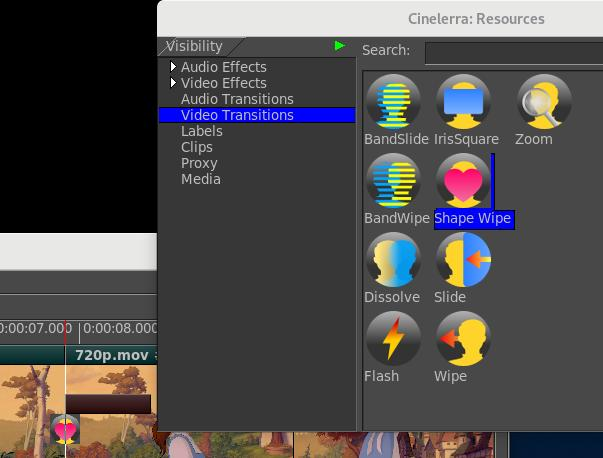
\includegraphics[width=0.8\linewidth]{images/transition.png}
    \caption{Resources window displaying the Video Transitions.}
    \label{fig:transition}
\end{figure}

Note the colored bar above the \textit{Shape Wipe} transition.

Transitions may only apply to the matching track type. Transitions under audio transitions can only apply to audio tracks. Transitions under video transitions can only apply to video tracks.

An example usage of a transition follows:
\begin{enumerate}
    \item Load a single video file and cut away a section from the center or make a blade cut so that you make two edits out of a single file. Make sure the edit boundary between the two edits is visible on the timeline.
    \item Go to the \textit{Resources window} and click on the \texttt{Video transitions} folder. Drag a transition from the transition list onto the second video edit on the timeline. A colored box highlights over where the transition will appear. Releasing over the $2^{nd}$ edit applies the transition between the $1^{st}$ and $2^{nd}$ edit.
\end{enumerate}
Once the transition is in place, it can be edited similarly to a plugin. Move the \textit{pointer} over the transition and \texttt{right click} to bring up the transition menu. The show option brings up specific parameters for the transition in question if any. The \texttt{length} option adjusts the length of the transition in seconds. The \texttt{detach} option removes the transition from the timeline. If the insertion point or the In point is over an edit, the beginning of the edit is covered by the transition.

Dragging and dropping transitions from the Resource window to the Program window can be tedious so there are shortcuts to solve this issue. Once you drag a transition from the Resources window, the \texttt{U} and \texttt{u} keys will paste the same transition. The U key pastes the last video transition and the u key pastes the last audio transition on all the recordable tracks. Another easy way to add the same transition to multiple edits is to get into \texttt{Arrow mode} (Drag and Drop editing), select the edits you would like to add the transition to and use the Video or Audio pulldown to \texttt{Attach transition}. Choose which transition you would like and click the checkmark \texttt{OK}. You can also set your default transition at any time by doing so in the Attach transition popup box – highlight your choice, and then at the bottom, click on the button \texttt{Set Default Transition}. You will see that name appear.

Transitions make two edits overlap for a certain amount of time. Cinelerra does not move edits during transitions. Instead it uses spare frames from the source file to lengthen the first edit enough to make it overlap the second edit for the duration of the transition. The exact point in time when the transition takes effect is the beginning of the second edit. The transition lasts a set amount of time into the second edit. For example, if you set a duration of 1 second for a dissolve transition, it will not start at the last 0.5 second of the first edit and continue 0.5 second into the second edit. In fact, it will start exactly at the beginning of the second edit and last for 1 second into that second edit. On the timeline a colored bar over the transition symbol visually represents the position and the duration of the transition.
The most important consequence of this behavior is that the first asset needs to have enough spare data after the end boundary to fill the transition into the second edit. Spare data duration should be equal or greater than the length of the transition effect set in the Length parameter of the transition popup menu.
If the last frame shown on the timeline is the last frame of the source file, Cinelerra will lengthen the first edit using the last frame only, with the unpleasant result of having the first edit freezing into the transition.

It should be noted that when playing transitions from the timeline to a hardware accelerated video device, the hardware acceleration will usually be turned \textit{off} momentarily during the transition and \textit{on} after the transition, in order to render the transition. Using an un-accelerated video device for the entire timeline normally removes the disturbance.

\section{Audio Transitions}%
\label{sec:audio_transition}

\subsection*{Crossfade}%
\label{sub:crossfade}

Creates a smooth transition from one audio source edit to another. The crossfade has the first source \textit{fade out} while the second \textit{fades in}.

\section{Video Transitions}%
\label{sec:video_transition}

In order to use a transition that you have dragged to the timeline, first right mouse click on the transition icon in the timeline. A menu will pop-up with the following controls:

\begin{description}
    \item[Show] Pops up the transition specific menu if available (not available on the dissolve transition).
    \item[On] Toggle on/off the transition effect.
    \item[Transition length] Set the length in seconds, frames, samples, \textit{H:M:S:frm} or \textit{H:M:S.xxx} for the transition to complete.  In addition you can use the mouse wheel to change the length in real time.
    \item[Detach] Remove the transition from the timeline.
\end{description}

\subsection*{BandSlide}%
\label{sub:bandslide}

Bands slide across video and you see the image slide.

\subsection*{BandWipe}%
\label{sub:bandwipe}

Bands wipe across the video and you see the mask slides.

\subsection{Flash}%
\label{sub:flash}

The video flashes when transitioning between segments.

\subsection*{IrisSquare}%
\label{sub:irissquare}

Video switches segments via a small rectangular view that gradually grows to full size.

\subsection*{Shape Wipe}%
\label{sub:shape_wipe}

Wipe a specific shape across the video. Currently available shapes are: \textit{burst}, \textit{circle}, \textit{clock}, \textit{heart}, \textit{specks}, \textit{spiral}, \textit{tile2x2h}, and \textit{tile2x2v}. 

You can add your own images to the Shape Wipe transition and there are some free ones available to download such as at \url{assistcg.com}.

To include new images in the Shape Wipe Transition, simply copy the file \texttt{{shape}.png} to your location of cinelerra in the subdirectory \texttt{plugins/shapes}.

\subsection*{Slide}%
\label{sub:slide}

Image slides into view; you can set \texttt{Left/Right/In/Out}.

\subsection*{Wipe}%
\label{sub:wipe}

Wipe the image across screen starting left or right.

\subsection*{Zoom}%
\label{sub:zoom}

Zoom out video at $\frac{X}{Y}$ magnification for some seconds.

